\begin{figure*}[[hbt!]]
\centering
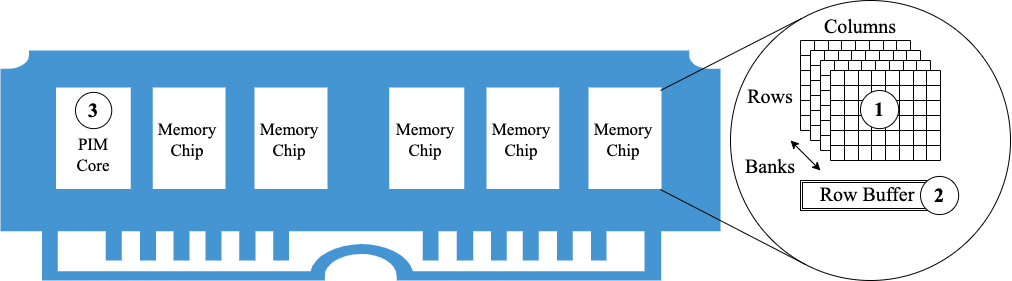
\includegraphics[width=.8\linewidth]{MEMSYS22/figures/pimcat.png}
%\vspace{.5em} 
\caption{Generic representation of a Main Memory DIMM and where processing in memory can take place.}
%\vspace{-1.5em} 
\label{fig:pimcat}
%\vspace{-0.6cm}    
\end{figure*}   
%\looseness -1




Processing in memory generally refers to the idea of moving some of the executions to the memory unit, when moving the data to the CPU for processing deem to take more time, which is often the case for memory intensive kernels. With various memory technologies and PIM optimization techniques present, there are several ways PIM can be adopted. Figure~\ref{fig:pimcat} shows a generic representation of a main memory DIMM module. A main memory DIMM (e.g. DDR4 DIMM) has several chips. Each chip has a number of banks (e.g. 4, 8, 16) and each bank has a specified number of rows and columns which constitutes the memory array (highlighted as \circled{1} in Figure ~\ref{fig:pimcat}). Each intersection of a row and column typically represents a memory \textit{cell} which holds single bit data. When a row address is requested to be accessed, that selected row is then loaded on to the row buffer (highlighted as \circled{2} in Figure ~\ref{fig:pimcat}). Several studies propose to use the memory array \circled{1} for computing \cite{03,06,13,15,20,29}, mostly for matrix vector multiplication operations where the coefficients can be mapped to the rows and columns to compute dot products using the array. The second category of PIM operations are proposed in the row buffer level \circled{2}; for example, by adding multiple row buffers and performing bit-wise operations among them \cite{31}. The third category of processing in memory suggests to have a simple processing unit near the memory banks capable of executing a sub-set of CPU instructions. The main intention of this model is to reduce memory traffic to/from CPU \cite{01,02,05,11,12,17,30,32,33,34,35}. 









%-	PIM background \\
%-	Different types of PIM \\
\textbf{-	Which type of PIM can be beneficial for HPC and why?} \\




  